
\serie{Conversions}

\begin{exercice}
Convertis les longueurs :
\begin{enumerate}
 \item $5$ mm = \ldots \ldots \ldots m ;
 \item $2,8$ hm = \ldots \ldots \ldots km ;
 \item $3$ dam = \ldots \ldots \ldots m ;
 \item $3,8$ dm = \ldots \ldots \ldots cm.
 \end{enumerate}
\end{exercice}


\begin{exercice}
Convertis dans l’unité demandée :
\begin{itemize}
 \item $\numprint{4405}$ m = \dotfill dam ;
 \item $0,007$ dam = \dotfill mm ;
 \item $45,3$ hm = \dotfill m ;
 \item $\numprint{12352}$ cm = \dotfill m ;
 \item $0,542$ km = \dotfill dm ;
 \item $7,03$ hm = \dotfill cm ;
 \item $\numprint{17005}$ cm = \dotfill km ;
 \item $123,5$ m = \dotfill km ;
 \item $0,045$ dam = \dotfill hm ;
 \item $\numprint{10000}$ mm =	\dotfill dam ;
 \item $6$ km $+ 12$ dam $+ 9$ m = \dotfill hm.
 \end{itemize}
\end{exercice}


\begin{exercice}
Pour aller au collège, Caroline fait d'abord 1,4 km avec son vélo qu'elle laisse chez sa grand‑mère. Puis elle parcourt les 150 m restant à pied. Quelle distance totale parcourt‑elle ?
\end{exercice}


\begin{exercice}
Recopie et complète :
\begin{enumerate}
 \item $4$ dam\up{2} = \ldots \ldots \ldots m\up{2} ;
 \item $15$ hm\up{2} = \ldots \ldots \ldots m\up{2} ;
 \item $5,1$ cm\up{2} = \ldots \ldots \ldots mm\up{2} ;
 \item $\numprint{1350}$ mm\up{2} = \ldots \ldots \ldots cm\up{2} ;
 \item $5,2$ km\up{2} = \ldots \ldots \ldots m\up{2} ;
 \item $0,7$ m\up{2} = \ldots \ldots \ldots dam\up{2} ;
 \item $320$ a = \ldots \ldots \ldots m\up{2} ;
 \item $2,5$ ha = \ldots \ldots \ldots m\up{2} ;
 \item $\numprint{15300}$ mm\up{2} = \ldots\ldots cm\up{2} =  \ldots\ldots dm\up{2} = \ldots\ldots m\up{2}.
 \end{enumerate}
\end{exercice}


\begin{exercice}
Convertis les aires suivantes en m\up{2} :
\begin{colenumerate}{3}
 \item $2$ km\up{2} ;
 \item $\numprint{37000}$ dm\up{2} ;
 \item $\numprint{45300}$ mm\up{2} ;
 \item $153,7$ dam\up{2} ;
 \item $28,9$ cm\up{2} ;
 \item $3,008$ hm\up{2} ;
 \item $52$ a ;
 \item $0,05$ ha ;
 \item $200$ ha.
 \end{colenumerate}
\end{exercice}


\begin{exercice}
Convertis les aires suivantes en cm\up{2} :
\begin{colenumerate}{3}
 \item $15$ mm\up{2} ;
 \item $28$ dm\up{2} ;
 \item $\numprint{17300}$ mm\up{2} ;
 \item $73,1$ m\up{2} ;
 \item $0,004$ m\up{2} ;
 \item $27,008$ dam\up{2} ;
 \item $0,08$ mm\up{2} ;
 \item $13$ a ;
 \item $\numprint{0,0105}$ a.
 \end{colenumerate}
\end{exercice}



%%%%%%%%%%%%%%%%%%%%%%%%%%Mise en page
\columnbreak
%%%%%%%%%%%%%%%%%%%%%%%%%%%%%%%%%%%%%%



\begin{exercice}
Convertis dans l’unité demandée :
\begin{itemize}
 \item $17$ cm = \ldots \ldots \ldots \ldots \ldots \ldots dm ;
 \item $17$ cm\up{2} = \ldots \ldots \ldots \ldots \ldots \ldots dm\up{2} ;
 \item $7,6$ km = \ldots \ldots \ldots \ldots \ldots \ldots dam ;
 \item $7,6$ km\up{2} = \ldots \ldots \ldots \ldots \ldots \ldots dam\up{2} ;
 \item $0,005$ dam\up{2} = \ldots \ldots \ldots \ldots \ldots \ldots m\up{2} ;
 \item $0,005$ dm\up{2} = \ldots \ldots \ldots \ldots \ldots \ldots m\up{2} ;
 \item $\numprint{12500}$ mm\up{2} = \ldots \ldots \ldots \ldots \ldots \ldots cm\up{2} ;
 \item $\numprint{12500}$ mm = \ldots \ldots \ldots \ldots \ldots \ldots cm ;
 \item $172$ a = \ldots \ldots \ldots \ldots \ldots \ldots ha ;
 \item $0,7$ dm\up{2} = \ldots \ldots \ldots \ldots \ldots \ldots a.
 \end{itemize}
\end{exercice}


\begin{exercice}
Range les aires suivantes dans l'ordre croissant. Justifie.

\begin{center} $5$ m\up{2} ; $\numprint{1360}$ mm\up{2} ; $0,08$ km\up{2} ; $91$ dam\up{2} ; $15$ cm\up{2}. \end{center}
\end{exercice}


%%%%%%%%%%%%%%%%%%%%%%%%%%Mise en page
\vspace{1em}
%%%%%%%%%%%%%%%%%%%%%%%%%%%%%%%%%%%%%%



%%%%%%%%%%%%%%%%%%%%%%%%%%%%%%%%%%%%%%%%%%%%%%%%%%%%%%%%%%%%%%%%%%%%

\serie{Avec un quadrillage}

\begin{exercice}
Détermine l'aire des figures suivantes :

\begin{center} 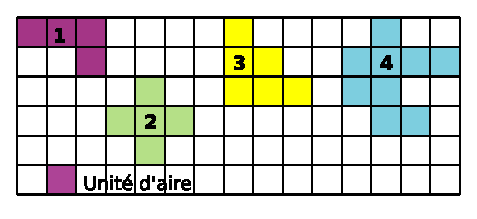
\includegraphics[width=7.2cm]{quadrillageA} \end{center}
\end{exercice}


\begin{exercice}
Détermine l'aire des figures suivantes :

\begin{center} 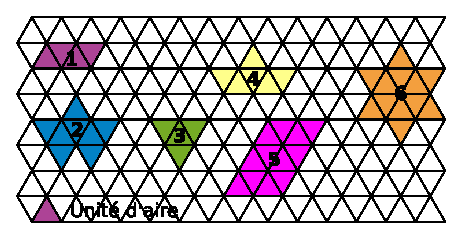
\includegraphics[width=6.9cm]{quadrillageB} \end{center}
\end{exercice}


\begin{exercice}
Détermine l'aire des triangles rectangles suivants :

\begin{center} 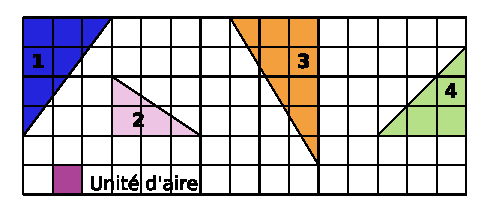
\includegraphics[width=7.2cm]{quadrillageC} \end{center}
\end{exercice}



%%%%%%%%%%%%%%%%%%%%%%%%%%Mise en page
\newpage
%%%%%%%%%%%%%%%%%%%%%%%%%%%%%%%%%%%%%%



\begin{exercice}
Détermine l'aire des triangles suivants :

\begin{center} 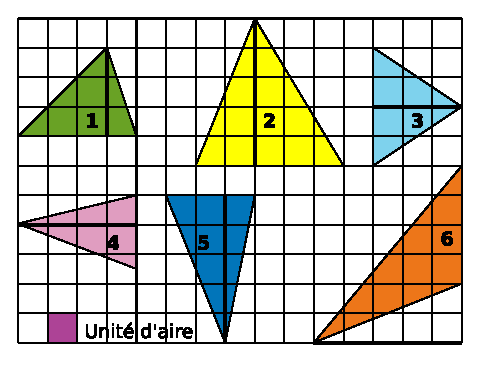
\includegraphics[width=7.2cm]{quadrillageD} \end{center}
\end{exercice}


\begin{exercice}
Détermine l'aire des figures suivantes :

\begin{center} 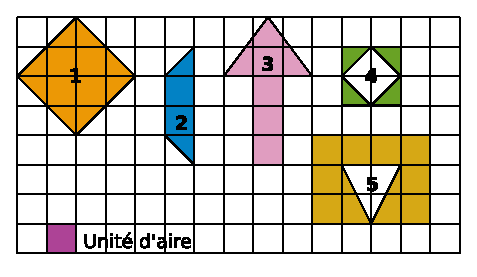
\includegraphics[width=7.1cm]{quadrillageE} \end{center}
\end{exercice}


\begin{exercice}
Détermine le périmètre des figures suivantes :

\begin{center} 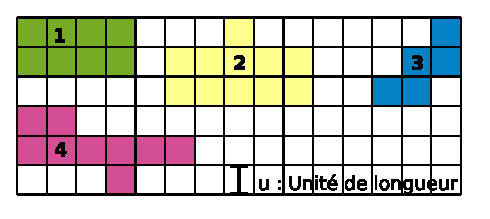
\includegraphics[width=7.1cm]{quadrillageF} \end{center}
\end{exercice}


\begin{exercice}[Avec les carreaux de ton cahier]
\begin{enumerate}
 \item En prenant comme unité d'aire un carreau de ton cahier, réalise trois figures différentes de cinq unités d'aire.
 \item Ces figures ont‑elles le même périmètre ?
 \end{enumerate}
\end{exercice}

\begin{exercice}[Avec les carreaux de ton cahier $(bis)$]
\begin{enumerate}
 \item En prenant comme unité de longueur la longueur d'un carreau de ton cahier, réalise trois figures différentes qui ont un périmètre de douze unités.
 \item Ces figures ont‑elles la même aire ?
 \end{enumerate}
\end{exercice}

\begin{exercice}[Comparaisons]
\begin{enumerate}
 \item Classe ces figures dans l'ordre croissant de leurs aires. Justifie.
 \item Classe ces figures dans l'ordre croissant de leurs périmètres.
 \item La figure qui a la plus grande aire a-t-elle également le plus grand périmètre ?
 \end{enumerate}
\begin{center} 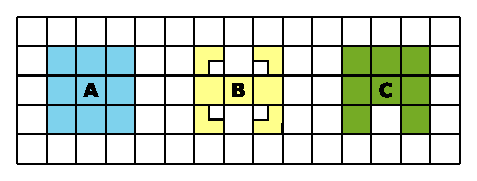
\includegraphics[width=7.1cm]{quadrillageG} \end{center}
\end{exercice}

\begin{exercice}[Aires approximatives]
\begin{center} 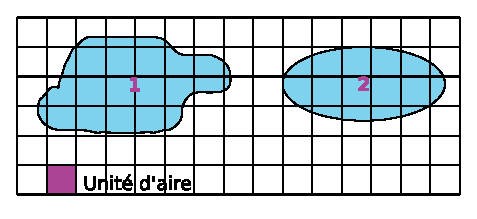
\includegraphics[width=7.2cm]{quadrillageH} \end{center}

Détermine un encadrement de l'aire de chacune des figures.
\end{exercice}


\begin{exercice}[Avec un quadrillage]
Sachant que l'unité d'aire est le carreau, détermine l'aire des figures suivantes en utilisant des aires de triangles :
\begin{center} 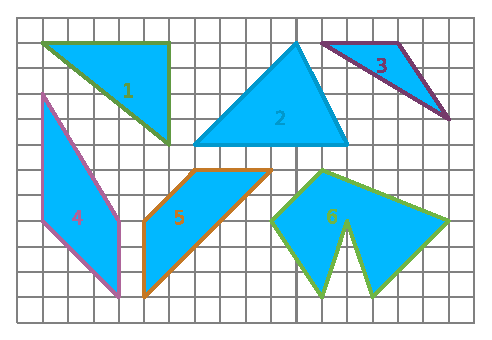
\includegraphics[width=7.1cm]{quadrillageL} \end{center} 
\end{exercice}



%%%%%%%%%%%%%%%%%%%%%%%%%%Mise en page
\newpage
%%%%%%%%%%%%%%%%%%%%%%%%%%%%%%%%%%%%%%



\begin{exercice}[Quadrillage]
\begin{center} 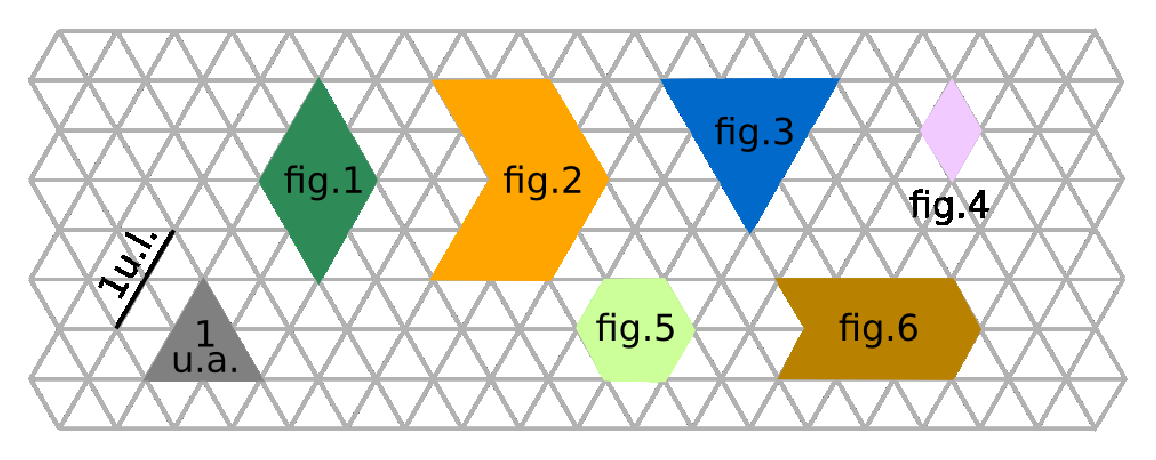
\includegraphics[width=\linewidth]{quadrillageM} \end{center}
\begin{enumerate}
 \item Sur la figure ci-dessus, après avoir observé l’unité de longueur choisie (1 u.l.), détermine le périmètre, en unité de longueur, de chaque figure :
 \begin{CLtableau}{\linewidth}{7}{c}
\hline
\textbf{Figure} & \textbf{1} & \textbf{2} & \textbf{3} & \textbf{4} & \textbf{5} & \textbf{6} \\\hline
\textbf{Périmètre}  & & & & & & \\
exprimé en u.l. & & & & & & \\\hline
 \end{CLtableau} 
 \item Après avoir observé l’unité d’aire choisie (1 u.a.), détermine l’aire, en unités d’aires, de chaque figure :
  \begin{CLtableau}{\linewidth}{7}{c}
\hline
\textbf{Figure} & \textbf{1} & \textbf{2} & \textbf{3} & \textbf{4} & \textbf{5} & \textbf{6} \\\hline
\textbf{Aire} & & & & & & \\
 exprimée en u.a. & & & & & & \\\hline
 \end{CLtableau} 
 \end{enumerate}
\end{exercice}


%%%%%%%%%%%%%%%%%%%%%%%%%%Mise en page
\vspace{1em}
%%%%%%%%%%%%%%%%%%%%%%%%%%%%%%%%%%%%%%




%%%%%%%%%%%%%%%%%%%%%%%%%%%%%%%%%%%%%%%%%%%%%%%%%%%%%%%%%%%%%%%%%%%%

\serie{Avec des formules}


\begin{exercice}[Périmètre et aire du carré]

Recopie et complète le tableau suivant où $c$ est la longueur du côté du carré, $\mathcal{P}$ son périmètre et $\mathcal{A}$ son aire :


\begin{ctableau}{\linewidth}{6}
\hline $c$  & 4 cm & 7 cm & 9 dm & & \\
\hline $\mathcal{P}$ & & & & 32 mm & \\
\hline  $\mathcal{A}$ & & & & & 36 m\up{2} \\
\hline
\end{ctableau}

\end{exercice}


\begin{exercice}[Calcul mental et rectangles]
Les mesures de cinq rectangles sont données en centimètres :

\begin{CLtableau}{\linewidth}{6}{c}
\hline
&  n\up{$\circ$} 1 &  n\up{$\circ$} 2 &  n\up{$\circ$} 3 &  n\up{$\circ$} 4 &  n\up{$\circ$} 5 \\
\hline Longueur & 3 & 5 & 8 & 9 & 8 \\
\hline Largeur & 2 & 3 & 6 & 7 & $1,5$ \\
\hline
\end{CLtableau}


\begin{enumerate}
 \item Calcule le périmètre de chaque rectangle ;
 \item Calcule l'aire de chaque rectangle.
 \end{enumerate}
\end{exercice}


\begin{exercice}[Calcul mental et triangles]
Les mesures des côtés de l'angle droit de cinq triangles rectangles sont données en centimètres :


\begin{cltableau}{\linewidth}{6}
\hline
  &  n\up{$\circ$} 1 & n\up{$\circ$} 2 &  n\up{$\circ$} 3 &  n\up{$\circ$} 4 &  n\up{$\circ$} 5 \\
\hline 1\up{er} côté & 3 & 5 & 8 & 9 & $1,5$ \\
\hline 2\up{ème} côté & 4 & 8 & 5 & 7 & $1,5$ \\
\hline
\end{cltableau}


Calcule l'aire de chaque triangle.
\end{exercice}



\begin{exercice}[Aire de triangles]
Calcule l'aire des différents triangles :
\begin{center} 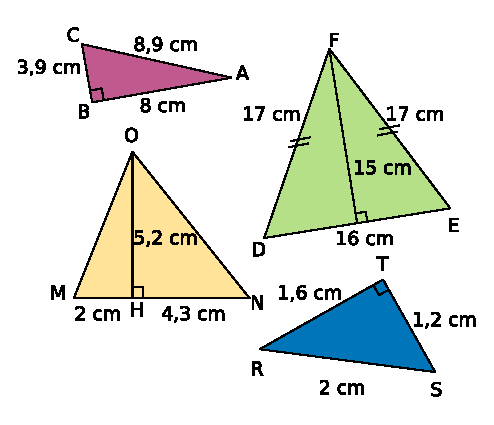
\includegraphics[width=7.6cm]{triangles_differents} \end{center}
\end{exercice}


\begin{exercice}[Aire de triangles rectangles]
Calcule l'aire des triangles rectangles suivants après en avoir fait un croquis :
\begin{enumerate}
 \item $ABC$ rectangle en $A$ tel que $AB = 5$ cm et $AC = 7$ cm ;
 \item $DEF$ rectangle en $E$ tel que $DF = 13$ cm, $DE = 5$ cm et $EF = 12$ cm ;
 \item $MNO$ d'hypoténuse $[MN]$ tel que $MN = 20$ mm, $MO = 12$ mm et $ON = 16$ mm.
 \end{enumerate}
\end{exercice}




%%%%%%%%%%%%%%%%%%%%%%%%%%Mise en page

\vspace*{2cm}

\phantom{Pour sauter une ligne}

\newpage
%%%%%%%%%%%%%%%%%%%%%%%%%%%%%%%%%%%%%%



\begin{exercice}[Périmètre de figures]
En prenant les mesures nécessaires, compare les périmètres des 6 figures ci‑dessous :

\begin{center} 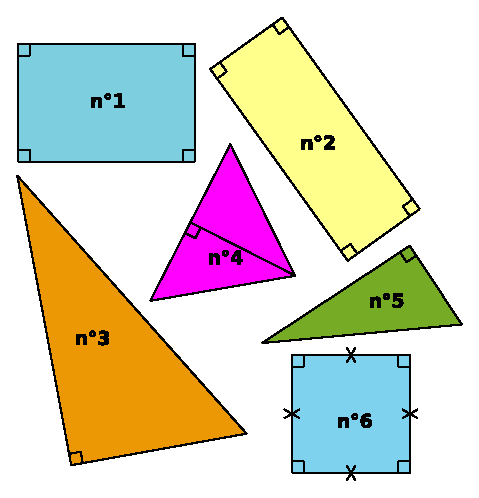
\includegraphics[width=7.4cm]{perimetre_figures} \end{center}
\end{exercice}


\begin{exercice}
Pour chaque parallélogramme, calcule la longueur demandée :
\begin{enumerate}
 \item L'aire du parallélogramme est 36 cm\up{2} et l'un de ses côtés mesure 6 cm. Combien mesure la hauteur relative à ce côté ?
 \item L'aire du parallélogramme est $15,12$ cm\up{2} et l'une de ses hauteurs mesure $3,6$ cm. Combien mesure la base relative à cette hauteur ?
 \end{enumerate}
\end{exercice}


\begin{exercice}[Avec un quadrillage]
Sachant que l'unité d'aire est le carreau, détermine l'aire de chaque figure suivante en utilisant des aires de parallélogrammes :

\begin{center} 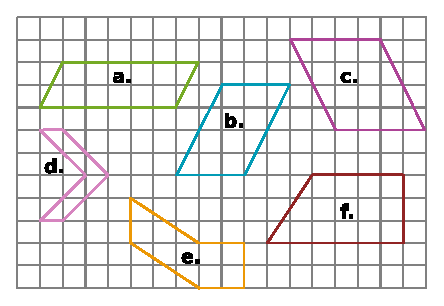
\includegraphics[width=6.6cm]{quadrillageI} \end{center}
\end{exercice}


\begin{exercice}[À main levée…]
\begin{minipage}[c]{0.48\linewidth}
Calcule l'aire et le périmètre de ce parallélogramme tracé à main levée. L'unité de longueur est le centimètre.
 \end{minipage} \hfill%
 \begin{minipage}[c]{0.48\linewidth}
\begin{center} 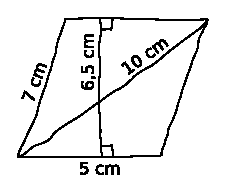
\includegraphics[width=2.9cm]{croquisJ} \end{center} 
  \end{minipage} \\
\end{exercice}


\begin{exercice}
Dans le tableau suivant, $c$ désigne un côté d'un parallélogramme, $h$ la hauteur relative à ce côté et $\mathcal{A}$ l'aire. Quelles sont les valeurs de E, F, G, H et I ? Justifie.

\begin{ltableau}{\linewidth}{3}
\hline
$c$ & $h$ & $\mathcal{A}$ \\\hline
$24$ cm & $8$ cm & E \\\hline
$132$ m & $0,5$ hm & F \\\hline
$16$ mm & G & $64$ mm\up{2} \\\hline
$4,5$ m & H & $14,4$ m\up{2} \\\hline
I & $250$ cm & $7,5$ m\up{2} \\\hline
 \end{ltableau} 
\end{exercice}


\begin{exercice}
Construis un parallélogramme qui a un côté de 6 cm de longueur, un périmètre de 20 cm et une aire de 18 cm\up{2}. Justifie ta construction en indiquant tes calculs.
\end{exercice}


\begin{exercice}[L'un dans l'autre]
\begin{enumerate}
 \item Calcule l'aire de $RATO$, sachant que $RA = 8$ cm et $AT = 6$ cm.
 \begin{center} 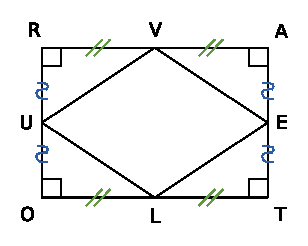
\includegraphics[width=4.2cm]{aireRATO} \end{center} 
 \item Calcule l'aire de $VELU$ de deux façons.
 \end{enumerate}
\end{exercice}


\begin{exercice}
Le quadrilatère $ABCD$ est un rectangle tel que $BC = 4$ cm, $AB = 6$ cm et $K$ est le milieu de $[AD]$. La surface colorée est formée de parallélogrammes accolés. Montre que l'aire de la surface colorée est la moitié de celle du rectangle.
 \begin{center} 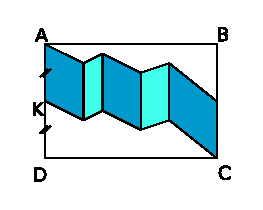
\includegraphics[width=3.6cm]{p_accoles} \end{center} 
\end{exercice}


\begin{exercice}[Pile ou Face ?]
\begin{minipage}[c]{0.38\linewidth}
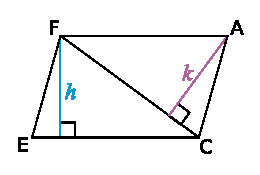
\includegraphics[width=3cm]{pile_face}
 \end{minipage} \hfill%
 \begin{minipage}[c]{0.58\linewidth}
Le parallélogramme $FACE$ est tel que :
 \begin{itemize}
  \item $EC = 150$ mm ;
  \item $h = 67$ mm ;
  \item $k = 53$ mm.
  \end{itemize}
  \end{minipage} \\
  \begin{enumerate}
   \item Calcule l'aire de $FACE$ ;
   \item Calcule la longueur de la diagonale $[FC]$.
   \end{enumerate}
\end{exercice}


\begin{exercice}[Avec ou sans quadrillage ?]
\begin{minipage}[c]{0.48\linewidth}
\begin{itemize}
 \item Recopie la figure, et partage-la en quatre triangles et un carré. Quelle est alors l'aire du parallélogramme $ABCD$ ?
 \end{itemize}
 \end{minipage} \hfill%
 \begin{minipage}[c]{0.48\linewidth}
\begin{center} 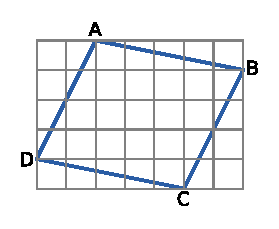
\includegraphics[width=3.7cm]{avec_sans} \end{center} 
  \end{minipage} \\
  \begin{itemize}
   \item Pourrais-tu trouver l'aire du parallélogramme $ABCD$ en utilisant seulement le quadrillage de côté $0,5$ cm ? 
   \end{itemize}
\end{exercice}


\begin{exercice}[Deux hauteurs]
\begin{minipage}[c]{0.48\linewidth}
Reproduis sur ton cahier la figure suivante puis trace en rouge la hauteur $[DH]$ et en vert la hauteur relative au côté $[DE]$.
 \end{minipage} \hfill%
 \begin{minipage}[c]{0.48\linewidth}
\begin{center} 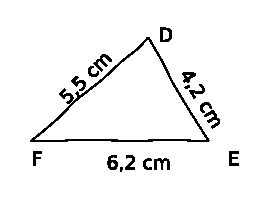
\includegraphics[width=3.3cm]{croquisFED} \end{center} 
  \end{minipage} \\
\end{exercice}


\begin{exercice}
Calcule l'aire du triangle $ABC$ ci-dessous de trois façons différentes en utilisant les informations données :

\begin{minipage}[c]{0.38\linewidth}
\begin{itemize}
 \item $AB = 12,5$ cm ;
 \item $BC = 20$ cm ;
 \item $AC = 19,5$ cm ;
 \item $CI = 18,72$ cm ;
 \item $AJ = 11,7$ cm ;
 \item $BK = 12$ cm.
 \end{itemize}
 \end{minipage} \hfill%
 \begin{minipage}[c]{0.58\linewidth}
\begin{center} 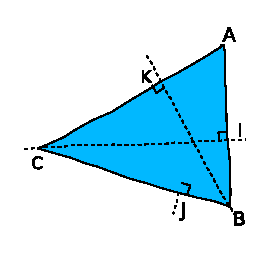
\includegraphics[width=3.6cm]{triangleKIJ} \end{center} 
  \end{minipage} \\
\end{exercice}



%%%%%%%%%%%%%%%%%%%%%%%%%%%%
\vfill
\columnbreak
%%%%%%%%%%%%%%%%%%%%%%%%%%%


\begin{exercice}
Calcule l'aire des triangles suivants. L'unité de longueur est le centimètre :
\begin{colenumerate}{2}
 \item 
 
 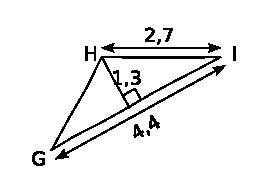
\includegraphics[width=3.1cm]{triangleAcm}
  \item 
 
 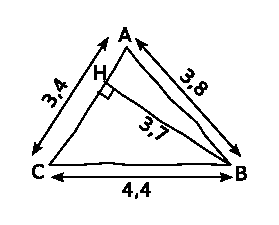
\includegraphics[width=3.5cm]{triangleBcm}
  \item 
 
 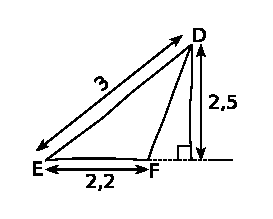
\includegraphics[width=3.3cm]{triangleCcm}
  \item 
 
 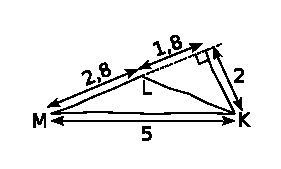
\includegraphics[width=3.5cm]{triangleDcm}
 \end{colenumerate}
\end{exercice}


\begin{exercice}
$MNP$ est un triangle de hauteur $[MH]$. Quels sont les valeurs de A, B, C ? Justifie.

\begin{center} 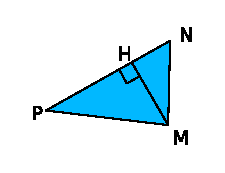
\includegraphics[width=2.5cm]{triangleHMNP} \end{center} 

\begin{ltableau}{\linewidth}{3}
\hline
\textbf{$NP$} & \textbf{$MH$} & \textbf{Aire du triangle $MNP$} \\\hline
$7,2$ cm & $4,8$ cm & A \\\hline
B & $3,5$ m & $5,6$ m\up{2} \\\hline
$16$ cm & C & $0,5$ dm\up{2} \\\hline
 \end{ltableau} 
\end{exercice}


\begin{exercice}
Un triangle a pour aire $16,25$ cm\up{2} et l'un de ses côtés mesure $6,5$ cm. Calcule la hauteur relative à ce côté.
\end{exercice}



\begin{exercice}
Un terrain rectangulaire de 45 m de long sur 28 m de large doit être entouré d’une clôture de 3 rangées de fil de fer. On prévoit une ouverture de 4 m de large.
\begin{enumerate}
 \item Quel est le périmètre de ce terrain ?
 \item Quelle est la longueur de fil de fer nécessaire ?
 \item Combien de rouleaux de 100 m de fil de fer faudra-t-il acheter ?
 \item Quelle est l’aire de ce terrain ? Donne la réponse en ares.
 \end{enumerate}
\end{exercice}




\begin{exercice}
Calcule l'aire des deux figures suivantes sans oublier de donner les formules :
\begin{center} \begin{tikzpicture}
%trapèze avec 2 angles droits marqués
\draw (0,0) node[below]{D} -- (7,0) node[below]{C} -- (5.5,3.5) node[above right]{B} -- (0,3.5) node [above left]{A} -- cycle;
\draw (0.2,0)|-(0,0.2);
\draw(0,3.3)-|(0.2,3.5);
\path (0,0) -- (0,3.5) node[midway, left]{3,5 cm};
\path (0,0) -- (7,0) node[midway,below]{7 cm};
\path (0,3.5) -- (5.5,3.5) node[midway,above]{5,5 cm};

\end{tikzpicture}
 \end{center} 
\begin{center} 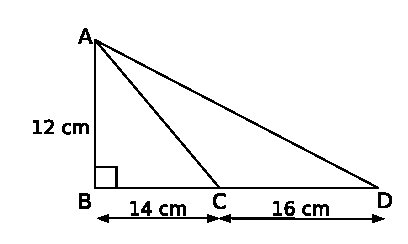
\includegraphics[width=5.8cm]{formule2} \end{center} 
\end{exercice}


\begin{exercice}
Le carré et le rectangle ci-dessous ont le même périmètre.
     
Après avoir fait tous les calculs nécessaires, calcule l’aire du carré.
\begin{center} 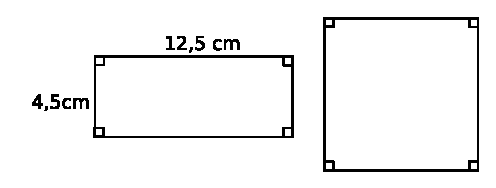
\includegraphics[width=7.2cm]{carre_rectangle} \end{center} 
\end{exercice}



%%%%%%%%%%%%%%%%%%%%%%%%%%%%%%%%%%%%%%%%%%%%%%%%%%%%%%%%%%%%%%%%%%%%
